\subsubsection{Bangui-Gruppe}\label{sec:BAN-Gr}

Neben Vertretern der durch die Roulettetechnick charakterisierten Stile Dama (Kap.~\ref{sec:DAM-Gr}) und Mbati-Ngombe (Kap.~\ref{sec:MBN-Gr}) wurden 1985 am Oberlauf des \mbox{Ubangi} auch eine Reihe von Gefäßen angekauft und bei Surveys gefunden, die keine Rouletteverzierung zeigen. Das als Bangui-Gruppe systematisierte Material setzt sich aus zehn GE zusammen, die sich an sieben verschiedenen Fundstellen fanden (Abb.~\ref{fig:BAN_Verbreitung}). Sicher der Bangui-Gruppe zurechenbare GE finden sich lediglich in einem kleinen Bereich zwischen Libenge im Süden (Fpl.~208) und Bangui im Norden (Fpl.~215). Eventuell der Stilgruppe zurechenbare Stücke fanden sich noch weiter flussauf, zwischen Gbandami (Fpl. 226) und \mbox{Kouango} (Fpl.~229). Neben den zwei in Balongoi (Fpl. 214; Abb.~\ref{fig:BAN_Typen}.1,4) und einer in Bangui angekauften GE (Fpl. 215; Abb.~\ref{fig:BAN_Typen}.3) stammen alle Stücke von Absammlungen rezenter Dorfflächen.

\paragraph{Technologische Merkmale}\hspace{-.5em}|\hspace{.5em}%
Die Scherben der Bangui-Keramik zeichnen sich durch einen geringeren Anteil nichtplastischer Partikel aus, die vornehmlich den Größenklassen \textit{fine} (43\,\%) sowie \textit{medium} (29\,\%) zuzurechnen sind. Die Anteile nichtplastischer Partikel im Scherben liegt in der Regel zwischen 3--5\,\% (57\,\%) und 7--10\,\% (29\,\%). Es handelt sich vornehmlich um heterogene Mischungen aus Quarz, Laterit und Glimmer. Vor allem der hohe Anteil von Glimmer in den Scherben ist auffällig. Aufgrund der kleinen Stichprobe können diese Zahlen selbstverständlich nur bedingt als repräsentativ angesehen werden. Mit Blick auf die \textit{Fabrics} ließen sich die Varianten 3c, 5c sowie 6b und 8a beobachten. Die Brennfarbe des genutzten Tons konnte in keinem Fall sicher bestimmt werden. Die Oberflächen der Stücke sind durchweg glatt, in einem Fall zeigt die Oberfläche sogar deutlich Hinweise auf eine intensive Glättung, welche als Politur angesprochen werden kann.

\begin{figure*}[p]
	\centering
	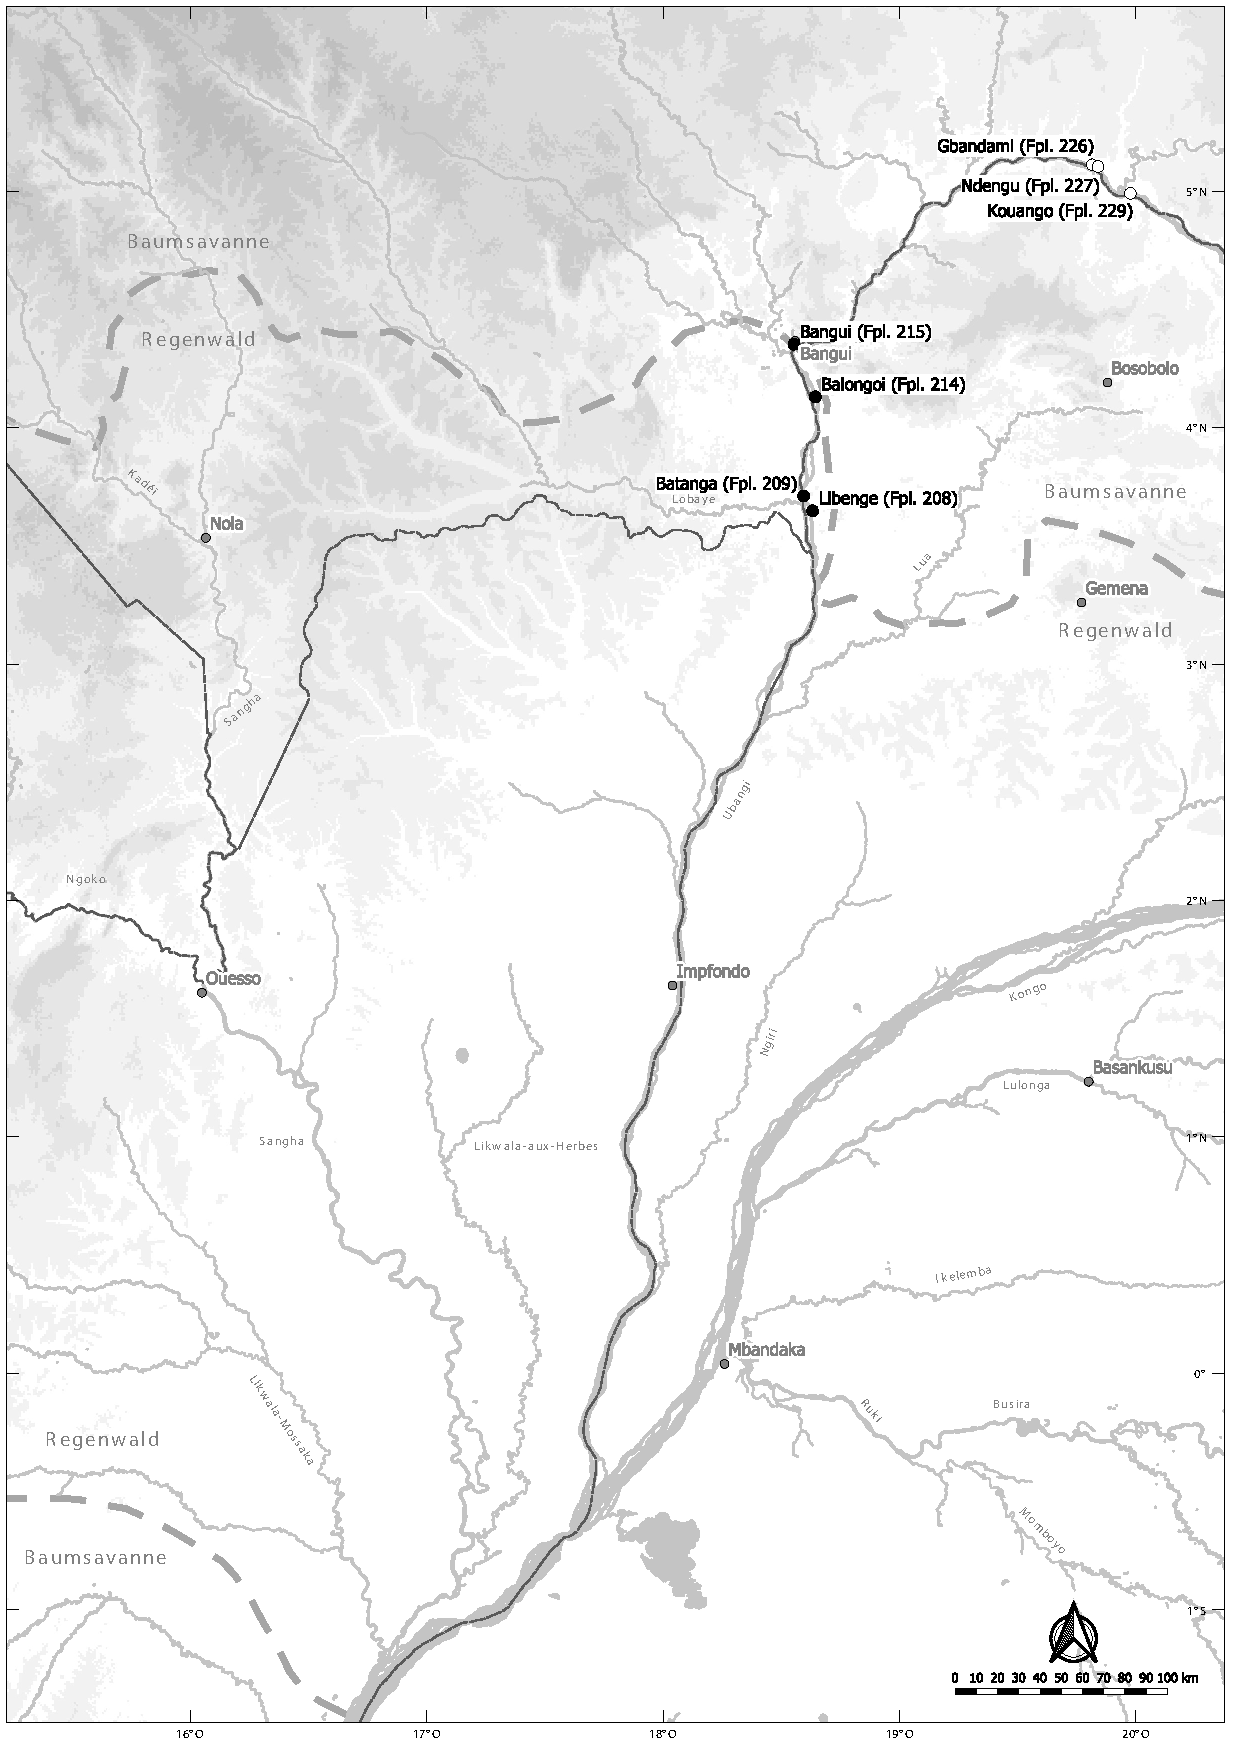
\includegraphics[width=\textwidth]{fig/BAN_Verbreitung.pdf}
	\caption{Bangui-Gruppe: Verbreitung.}
	\label{fig:BAN_Verbreitung}
\end{figure*}

\paragraph{Formen}\hspace{-.5em}|\hspace{.5em}%
Lediglich bei sechs der zehn GE der Bangui-Gruppe war eine Ansprache der Gefäßform möglich. Vier GE sind flache Gefäße mit geschweifter Wandung (Typ~E; Abb.~\ref{fig:BAN_Typen}.3--4). Ebenfalls vertreten ist ein flaschenförmiges Gefäß (Typ~A; Abb.~\ref{fig:BAN_Typen}.1) sowie ein schalenförmiges Gefäß mit konvexer Wandung (Typ~I; Taf.~24.2). Die Randlippen sind etwa zu gleichen Anteilen rund (M1), spitz (M2) oder gerade (M3) ausgearbeitet, während die Ausrichtung der Ränder grundsätzlich ausbiegend ist. Gerade (B1) sowie konkav (B2) oder konvex ausbiegende Ränder (B3) kommen etwa zu gleichen Anteilen vor. Die Halsbereiche der Gefäße sind häufig sehr kurz gehalten oder überhaupt nicht dezidiert ausgearbeitet. Bei vier GE konnte die Ausprägung des Bodens beobachtet werden. Neben zwei runden Böden (B1; Abb.~\ref{fig:BAN_Typen}.4; Taf.~24.8) wurden auch zwei flache Standböden (B4; Abb.~\ref{fig:BAN_Typen}.1,3) beobachtet.

\paragraph{Verzierungen}\hspace{-.5em}|\hspace{.5em}%
Die GE der Bangui-Gruppe zeichnen sich durch eine klare Strukturierung ihrer Verzierung aus. Auf den Unterseiten sowie Standflächen findet sich eine flächige, an \textit{banfwa-nfwa} (Tab.~\ref{tab:Verzierungselemente}: 08) erinnernde aber stellenweise auffällig irreguläre Aufrauung der Oberfläche (Tab.~\ref{tab:Verzierungselemente}: 22.2; 27\,\%; Abb.~\ref{fig:BAN_Typen}.1--3). Die oberen Gefäßteile zeichnen sich regelhaft durch horizontale Bänder runder bis leicht ovaler Eindrücke (Tab.~\ref{tab:Verzierungselemente}: 04.11; 24\,\%; Abb.~\ref{fig:BAN_Typen}.1--4) sowie horizontaler Riefen aus (Tab.~\ref{tab:Verzierungselemente}: 02.1; 26\,\%; Abb.~\ref{fig:BAN_Typen}.4).\footnote{Diese Verzierung der Gefäßoberteile durch horizontale Bänder erinnert an die Verzierungspraxis der Kpetene-Gruppe (Kap.~\ref{sec:KPT-Gr}).} Die Eindrücke können auch größere geometrische Flächen ausfüllen (Abb.~\ref{fig:BAN_Typen}.1). Ebenso ließen sich Kombinationen aus horizontalen (Tab.~\ref{tab:Verzierungselemente}: 02.1) sowie winkelförmig ausgearbeiteten Riefen-Bändern beobachten (Tab.~\ref{tab:Verzierungselemente}: 01.6 und 02.3; Abb.~\ref{fig:BAN_Typen}.3).\footnote{Die auf einer GE (Abb.~\ref{fig:BAN_Typen}.4) beobachteten bogenförmigen Riefen könnten auf eine Beziehung der Bangui-Keramik zur Mokelo-Gruppe (Kap.~\ref{sec:MKL-Gr}) hinweisen.}


\paragraph{Datierung}\hspace{-.5em}|\hspace{.5em}%
Absolute Daten für die chronologische Ansprache der Keramik des Bangui-Stils liegen nicht vor. Die beiden in Balongoi (Fpl.~214; Abb.~\ref{fig:BAN_Typen}.1,4) sowie die in Bangui (Fpl. 215; Abb.~\ref{fig:BAN_Typen}.3) als \textit{Ethnographica} angekauften GE belegen jedoch die rezente Nutzung der Gefäße und legen ein grundsätzlich zeitgenössisches Alter nahe.

Die morphologischen Eigenschaften der Bangui-Gruppe erinnern mit Blick auf die grundsätzlich rundbauchigen Gefäße, das Fehlen ausgeprägter Hals"-partien sowie das Vorhandensein kurzer, ausbiegender Ränder an die Dama-Keramik (Kap.~\ref{sec:DAM-Gr}). Die flächige \textit{Behandlung} beziehungsweise Aufrauung der Gefäßunterseiten stellt eine Parallele zur Kpetene-Gruppe dar (Kap.~\ref{sec:KPT-Gr}). Die Bänder aus Eindrücken hingegen stellen einen Bezug zur älteren Keramik der Mokelo-Gruppe (Kap.~\ref{sec:MKL-Gr}) her, die etwa in der gleichen Region verbreitet ist (Abb.~\ref{fig:MKL_Verbreitung}).

\paragraph{Verbreitung}\hspace{-.5em}|\hspace{.5em}%
Bangui-Keramik findet sich in einem kleinen Verbreitungsgebiet direkt südlich der Hauptstadt der Zentralafrikanischen Republik Bangui, die der eponyme Fundplatz für die Stilgruppe ist (Fpl.~215). Der südlichste Fundplatz von sicher als Bangui ansprechbarer Keramik ist Libenge (Fpl.~208), während der nördlichste Bangui selbst ist. Etwa 160\,km stromauf von Bangui, kurz vor dem Ende der Befahrung von 1985, fanden sich zwischen Gbandami (Fpl.~226) und Kou"-a"-ngo (Fpl.~229) GE, die möglicherweise der Bangui-Gruppe zuzuweisen sind. Eine Erklärung dieses Verbreitungsbildes kann, beruhend auf der gegenwärtig vorliegenden, sehr begrenzten empirischen Datenlage, nicht gegeben werden.\footnote{Das engere Verbreitungsgebiet zwischen Libenge (Fpl.~208) und Bangui (Fpl.~215) könnte mit begrenztem Handel der Stücke erklärt werden.}